\documentclass[11pt]{article}
\usepackage{xcolor}
\usepackage{times}
\usepackage{amsthm}
\usepackage{amssymb}
\usepackage{amsmath}
\usepackage{multirow}
\usepackage{array}
\usepackage{graphicx}
\usepackage[linesnumbered,ruled,vlined]{algorithm2e}
\usepackage[czech]{babel}
\usepackage[IL2]{fontenc}
\usepackage[a4paper,total={17cm,24cm},left=2cm,top=3cm]{geometry}
\usepackage[colorlinks=true,linkcolor=black,urlcolor=black]{hyperref}
\theoremstyle{plain}
\newtheorem{definition}{Definice}
\theoremstyle{plain}
\newtheorem{theorem}{Věta}
\begin{document}
\begin{titlepage}
    \begin{center}
        {\textsc{{\Huge Vysoké učení technické v Brně\\[0.5em]\huge{Fakulta informačních technologií}}\\}}
        \vspace{\stretch{0.382}}
        {\LARGE{Typografie a publikování\,--\,3. projekt}\\[0.4em]}
        {\LARGE{Tabulky a obrázky}}
        \vspace{\stretch{0.618}}
    \end{center}
    {\Large 20. března 2023 \hfill Josef Kuchař}
\end{titlepage}
\clearpage

\section{Úvodní strana}
Název práce umístěte do zlatého řezu a nezapomeňte uvést \uv{dnešní} (today) datum a vaše jméno a příjmení.

\section{Tabulky}
Pro sázení tabulek můžeme použít buď prostředí \verb|tabbing| nebo prostředí \verb|tabular|.

\subsection{Prostředí \texttt{tabbing}}
Při použití \verb|tabbing| vypadá tabulka následovně:

\begin{tabbing}
    \hspace{7em} \= \hspace{3em} \= \kill
    \textbf{Ovoce} \> \textbf{Cena} \> \textbf{Množství} \\
    Jablka \> 25,90 \> 3 kg \\
    Hrušky \> 27,40 \> 2,5 kg \\
    Vodní melouny \> 35,-- \> 1 kus \\
\end{tabbing}
Toto prostředí se dá také použít pro sázení algoritmů, ovšem vhodnější je použít prostředí \verb|algorithm| nebo \verb|algorithm2e| (viz sekce 3).

\subsection{Prostředí \texttt{tabular}}
Další možností, jak vytvořit tabulku, je použít prostředí \verb|tabular|. Tabulky pak budou vypadat takto\footnote{Kdyby byl problém s cline, zkuste se podívat třeba sem: \url{http://www.abclinuxu.cz/tex/poradna/show/325037}.}:

\begin{table}[h]
    \catcode`\-=12
    \begin{center}
        \begin{tabular}{|l|c|c|}
            \hline
                          & \multicolumn{2}{|c|}{\textbf{Cena}}                   \\
            \cline{2-3}
            \textbf{Měna} & \textbf{nákup}                      & \textbf{prodej} \\
            \hline
            EUR           & 22,705                              & 25,242          \\
            GBP           & 25,931                              & 28,828          \\
            USD           & 21,347                              & 23,732          \\
            \hline
        \end{tabular}
        \caption{Tabulka kurzů k dnešnímu dni}
    \end{center}
\end{table}

\begin{table}[h]
    \catcode`\-=12
    \begin{tabular}{|c|c|}
        \hline
        $A$        & $\neg A$ \\
        \hline
        \textbf{P} & N        \\
        \hline
        \textbf{O} & O        \\
        \hline
        \textbf{X} & X        \\
        \hline
        \textbf{N} & P        \\
        \hline
    \end{tabular}
    % \hline
    % \multicolumn{2}{|c|}{\multirow{2}{*}{$A$}} & \multicolumn{4}{|c|}{$B$}                                        \\
    % \cline{3-6}

    \caption{Protože Kleeneho trojhodnotová logika už je \uv{zastaralá}, uvádíme si zde příklad čtyřhodnotové logiky}
\end{table}

% \begin{tabular}[|c|c|c|c|]
%     \hline
%     \textbf{P} & \textbf{O} & \textbf{X} & \textbf{N} \\
% \end{tabular}

\section{Algoritmy}
Pokud budeme chtít vysázet algoritmus, můžeme použít prostředí \verb|algorithm|\footnote{Pro nápovědu, jak zacházet s prostředím algorithm, můžete zusit tuhle stránku: \url{http://ftp.cstug.cz/pub/tex/CTAN/macros/latex/contrib/algorithms/algorithms.pdf}.}
nebo \verb|algorithm2e|\footnote{Pro algorithm2e zase tuhle: \url{http://ftp.cstug.cz/pub/tex/CTAN/macros/latex/contrib/algorithm2e/doc/algorithm2e.pdf}.}.
Příklad použití prostředí \verb|algorithm2e| viz Algoritmus 1.

\SetAlgoNoLine
\begin{algorithm}
    \caption{\textsc{Fast}SLAM}
    \KwIn{$(X_{t-1}, u_t, z_t)$}
    \KwOut{$X_t$}
    $\overline{X_t} + X_t = 0$ \\
    \For{$k = 1$ \emph{to} $M$}{
        $x^{[k]}_t = sample\_motion\_model(u_t, x^{[k]}_{t-1})$ \\
        $\omega^{[k]}_t = measurement\_model(z_t, x^{[k]}_t, m_{t-1})$ \\
        $m^{[k]}_t = updated\_occupancy\_grid(z_t, x^{[k]}_t, m^{[k]}_{t-1})$ \\
        $\overline{X_t} = \overline{X_t} + \langle x^{[m]}_x, \omega^{[m]}_t \rangle$ \\
    }
    \For{$k = 1$ \emph{to} $M$}{
        draw $i$ with probability $\approx \omega^{[i]}_t$\\
        add $\langle x^{[k]}_x, m^{[k]}_t\rangle$ to $X_t$
    }
    \Return{$X_t$}
\end{algorithm}

\section{Obrázky}
Do našich článků můžeme samozřejmě vkládat obrázky. Pokud je obrázkem fotografie, můžeme klidně použít bitmapový soubor. Pokud by to ale mělo být nějaké schéma, nebo něco podobného, je dobrým zvyktem takovýto obrázek vytvořit vektorově.

\begin{figure}[h]
    \centering
    \scalebox{0.33}{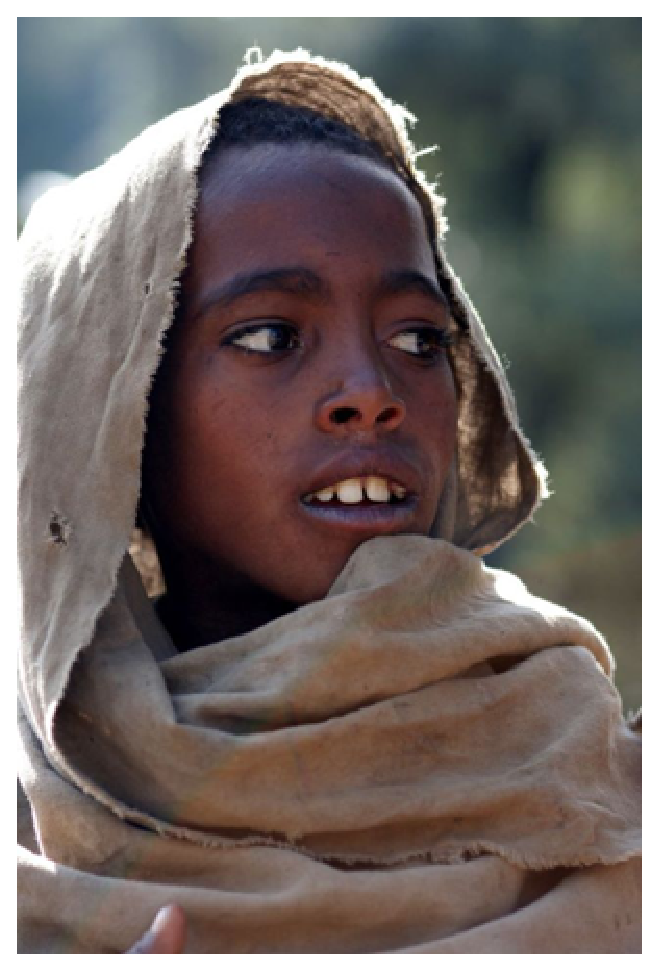
\includegraphics{etiopan.eps}
        \reflectbox{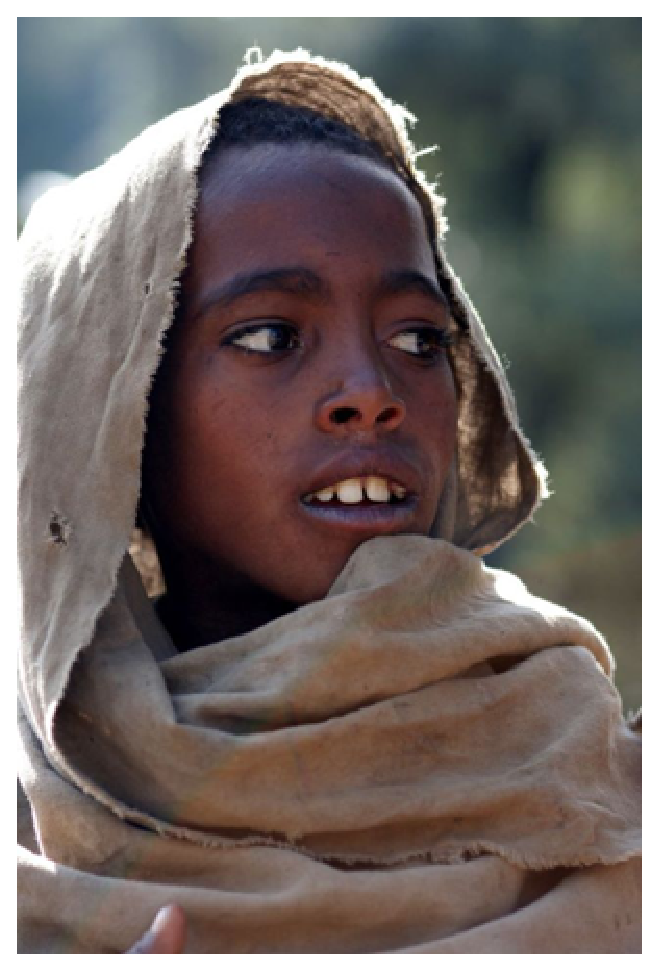
\includegraphics{etiopan.eps}} }
    \caption{Malý Etiopánek a jeho bratříček}
\end{figure}

Rozdíl mezi vektorovým \dots

\begin{figure}[h]
    \centering
    
\includegraphics[width=0.5\textwidth]{oniisan.eps}
    \caption{Vektorový obrázek}
\end{figure}

\dots a bitmapovým obrázkem

\begin{figure}[h]
    \centering
    
\includegraphics[width=0.5\textwidth]{oniisan2.eps}
    \caption{Bitmapový obrázek}
\end{figure}

se projeví například při zvětšení.

Odkazy (nejen ty) na obrázky 1, 2 a 3, na tabulky 1 a 2 a také algoritmus 1 jsou udělány pomocí křížových odkazů. Pak je ovšem potřeba zdrojový soubor přeložit dvakrát.

Vektorové obrázky lze vytvořit i přímo v \LaTeX um, například pomocí prostředí \verb|picture|.

\end{document}
